\documentclass{standalone}
\usepackage{tkz-fct}
\usepackage{tkz-euclide}
\usepackage{amsmath}
\usepackage{color}
\renewcommand*\familydefault{\sfdefault}
\usepackage{sansmath}
\sansmath
\definecolor{gray75}{gray}{0.75}
\begin{document}
 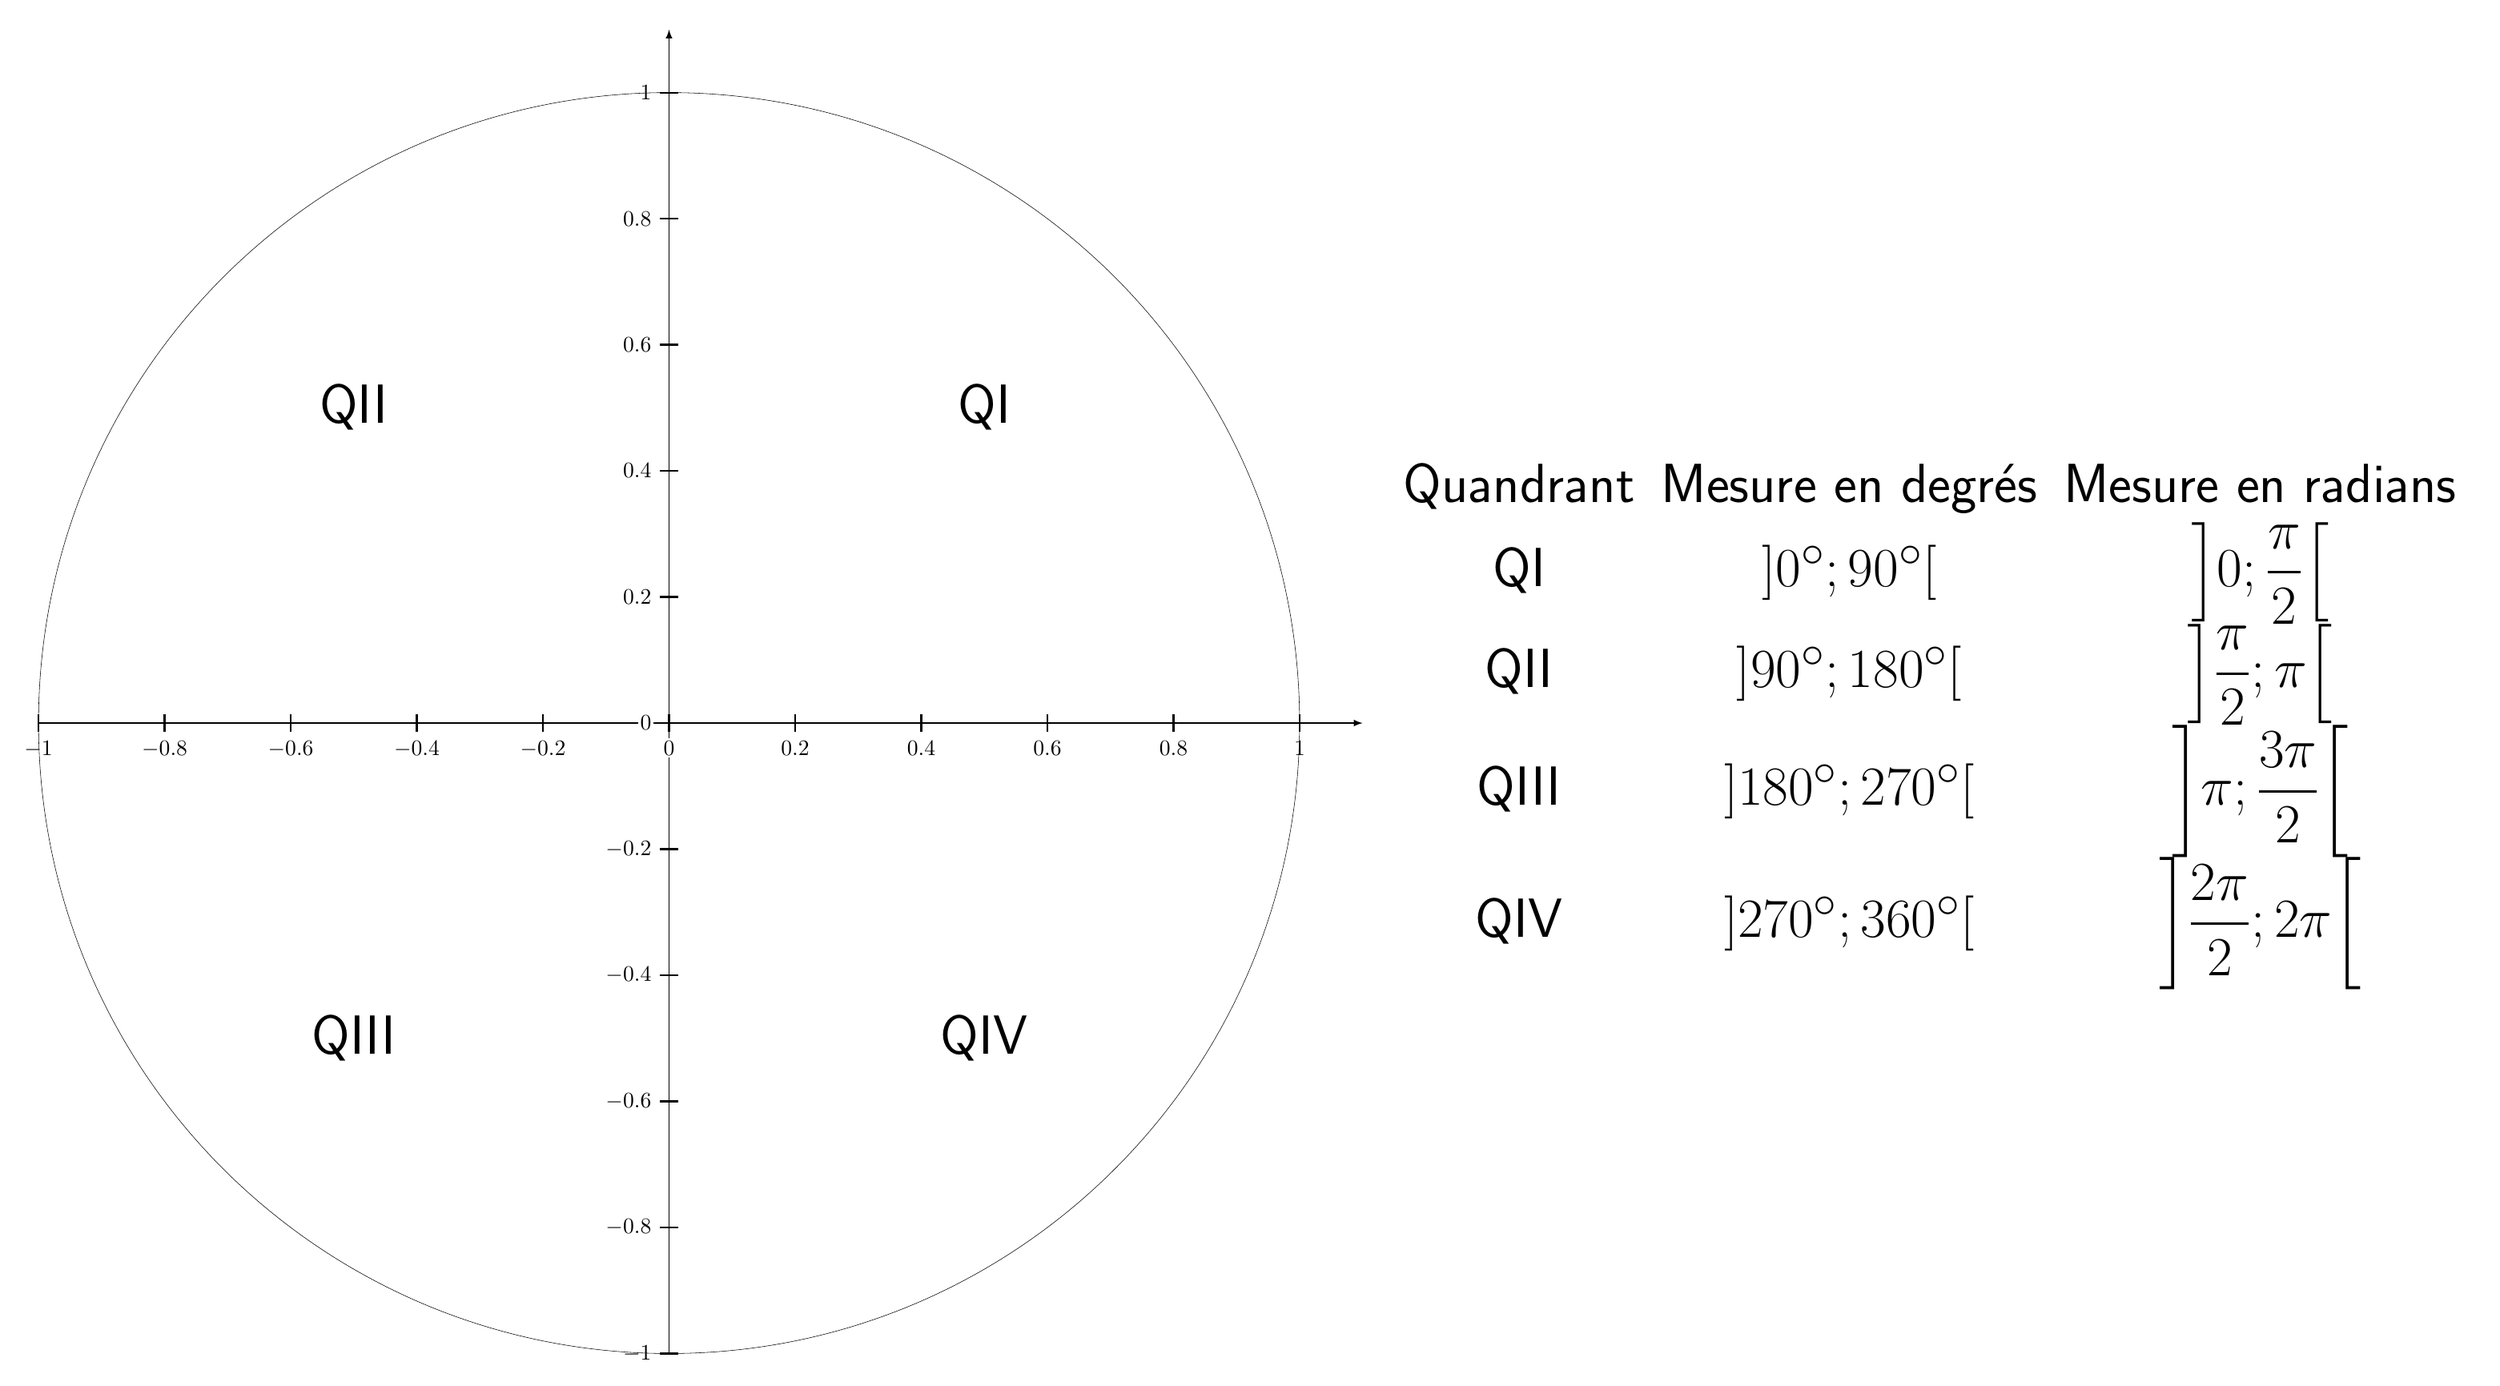
\begin{tikzpicture}[scale=2]
   \tkzInit[xmax=1.,ymax=1.,xmin=-1. ,ymin=-1,xstep=0.2,ystep=0.2]
   \tkzAxeXY[label={}]
   % \begin{scope}[dashed]
   %   \tkzGrid
   % \end{scope}

   \tkzDefPoints{0/0/O,1/0/A}
   \tkzDrawCircle[color=black](O,A)
\tkzText(.5,.5){\Huge QI}
\tkzText(-.5,.5){\Huge QII}
\tkzText(-.5,-.5){\Huge QIII}
\tkzText(.5,-.5){\Huge QIV}
\tkzText(2,0){\Huge
\begin{tabular}{ccc}
Quandrant & Mesure en degrés        & Mesure en radians                   \\
QI        & $]0^\circ;90^\circ[$    & $\left]0;\dfrac{\pi}{2}\right[$     \\
QII       & $]90^\circ;180^\circ[$  & $\left]\dfrac{\pi}{2};\pi\right[$   \\
QIII      & $]180^\circ;270^\circ[$ & $\left]\pi;\dfrac{3\pi}{2}\right[$  \\
QIV       & $]270^\circ;360^\circ[$ & $\left]\dfrac{2\pi}{2};2\pi\right[$
\end{tabular}
}
\end{tikzpicture}
\end{document}
